% !TEX TS-program = xelatex
% !TEX encoding = UTF-8 Unicode
% !Mode:: "TeX:UTF-8"

\documentclass{resume}
\usepackage{zh_CN-Adobefonts_external} % Simplified Chinese Support using external fonts (./fonts/zh_CN-Adobe/)
%\usepackage{zh_CN-Adobefonts_internal} % Simplified Chinese Support using system fonts
\usepackage{linespacing_fix} % disable extra space before next section
\usepackage{cite}

% 统一字体：正文、标题、联系方式统一使用同一字体风格
\setCJKsansfont{AdobeSongStd-Light.otf}
\setCJKmonofont{AdobeSongStd-Light.otf}
\renewcommand{\familydefault}{\rmdefault}
\titleformat{\section}{\Large\bfseries\raggedright}{}{0em}{}[\titlerule]
\titleformat{\subsection}{\large\raggedright}{}{0em}{}
\renewcommand{\name}[1]{
  \centerline{\Huge\bfseries{#1}}
  \vspace{1.2ex}
}
\renewcommand{\contactInfo}[4]{
  \centerline{\large{\ {#1} \textperiodcentered\ \ {#2}}
    \ifthenelse{\isempty{#3}}{ }{\textperiodcentered\ \ {#3} }
    \ifthenelse{\isempty{#4}}{ }{\textperiodcentered\ \ {#4} }
  }
  \vspace{0.7ex}
}

\begin{document}
\pagenumbering{gobble} % suppress displaying page number

\vspace*{-15pt}
\noindent
\begin{minipage}[t]{0.82\textwidth}
  \name{王洋}
  \contactInfo{男 | 26岁 | 武汉}{电话： 15623362892}{邮箱： 1439256987@qq.com}{}
  {\small\centering 个人主页：\texttt{brown-yang.github.io} \textperiodcentered\ 研究方向：具身智能、AI\par}
\end{minipage}
\hfill
\begin{minipage}[t]{0.15\textwidth}
  \vspace{-40pt}
  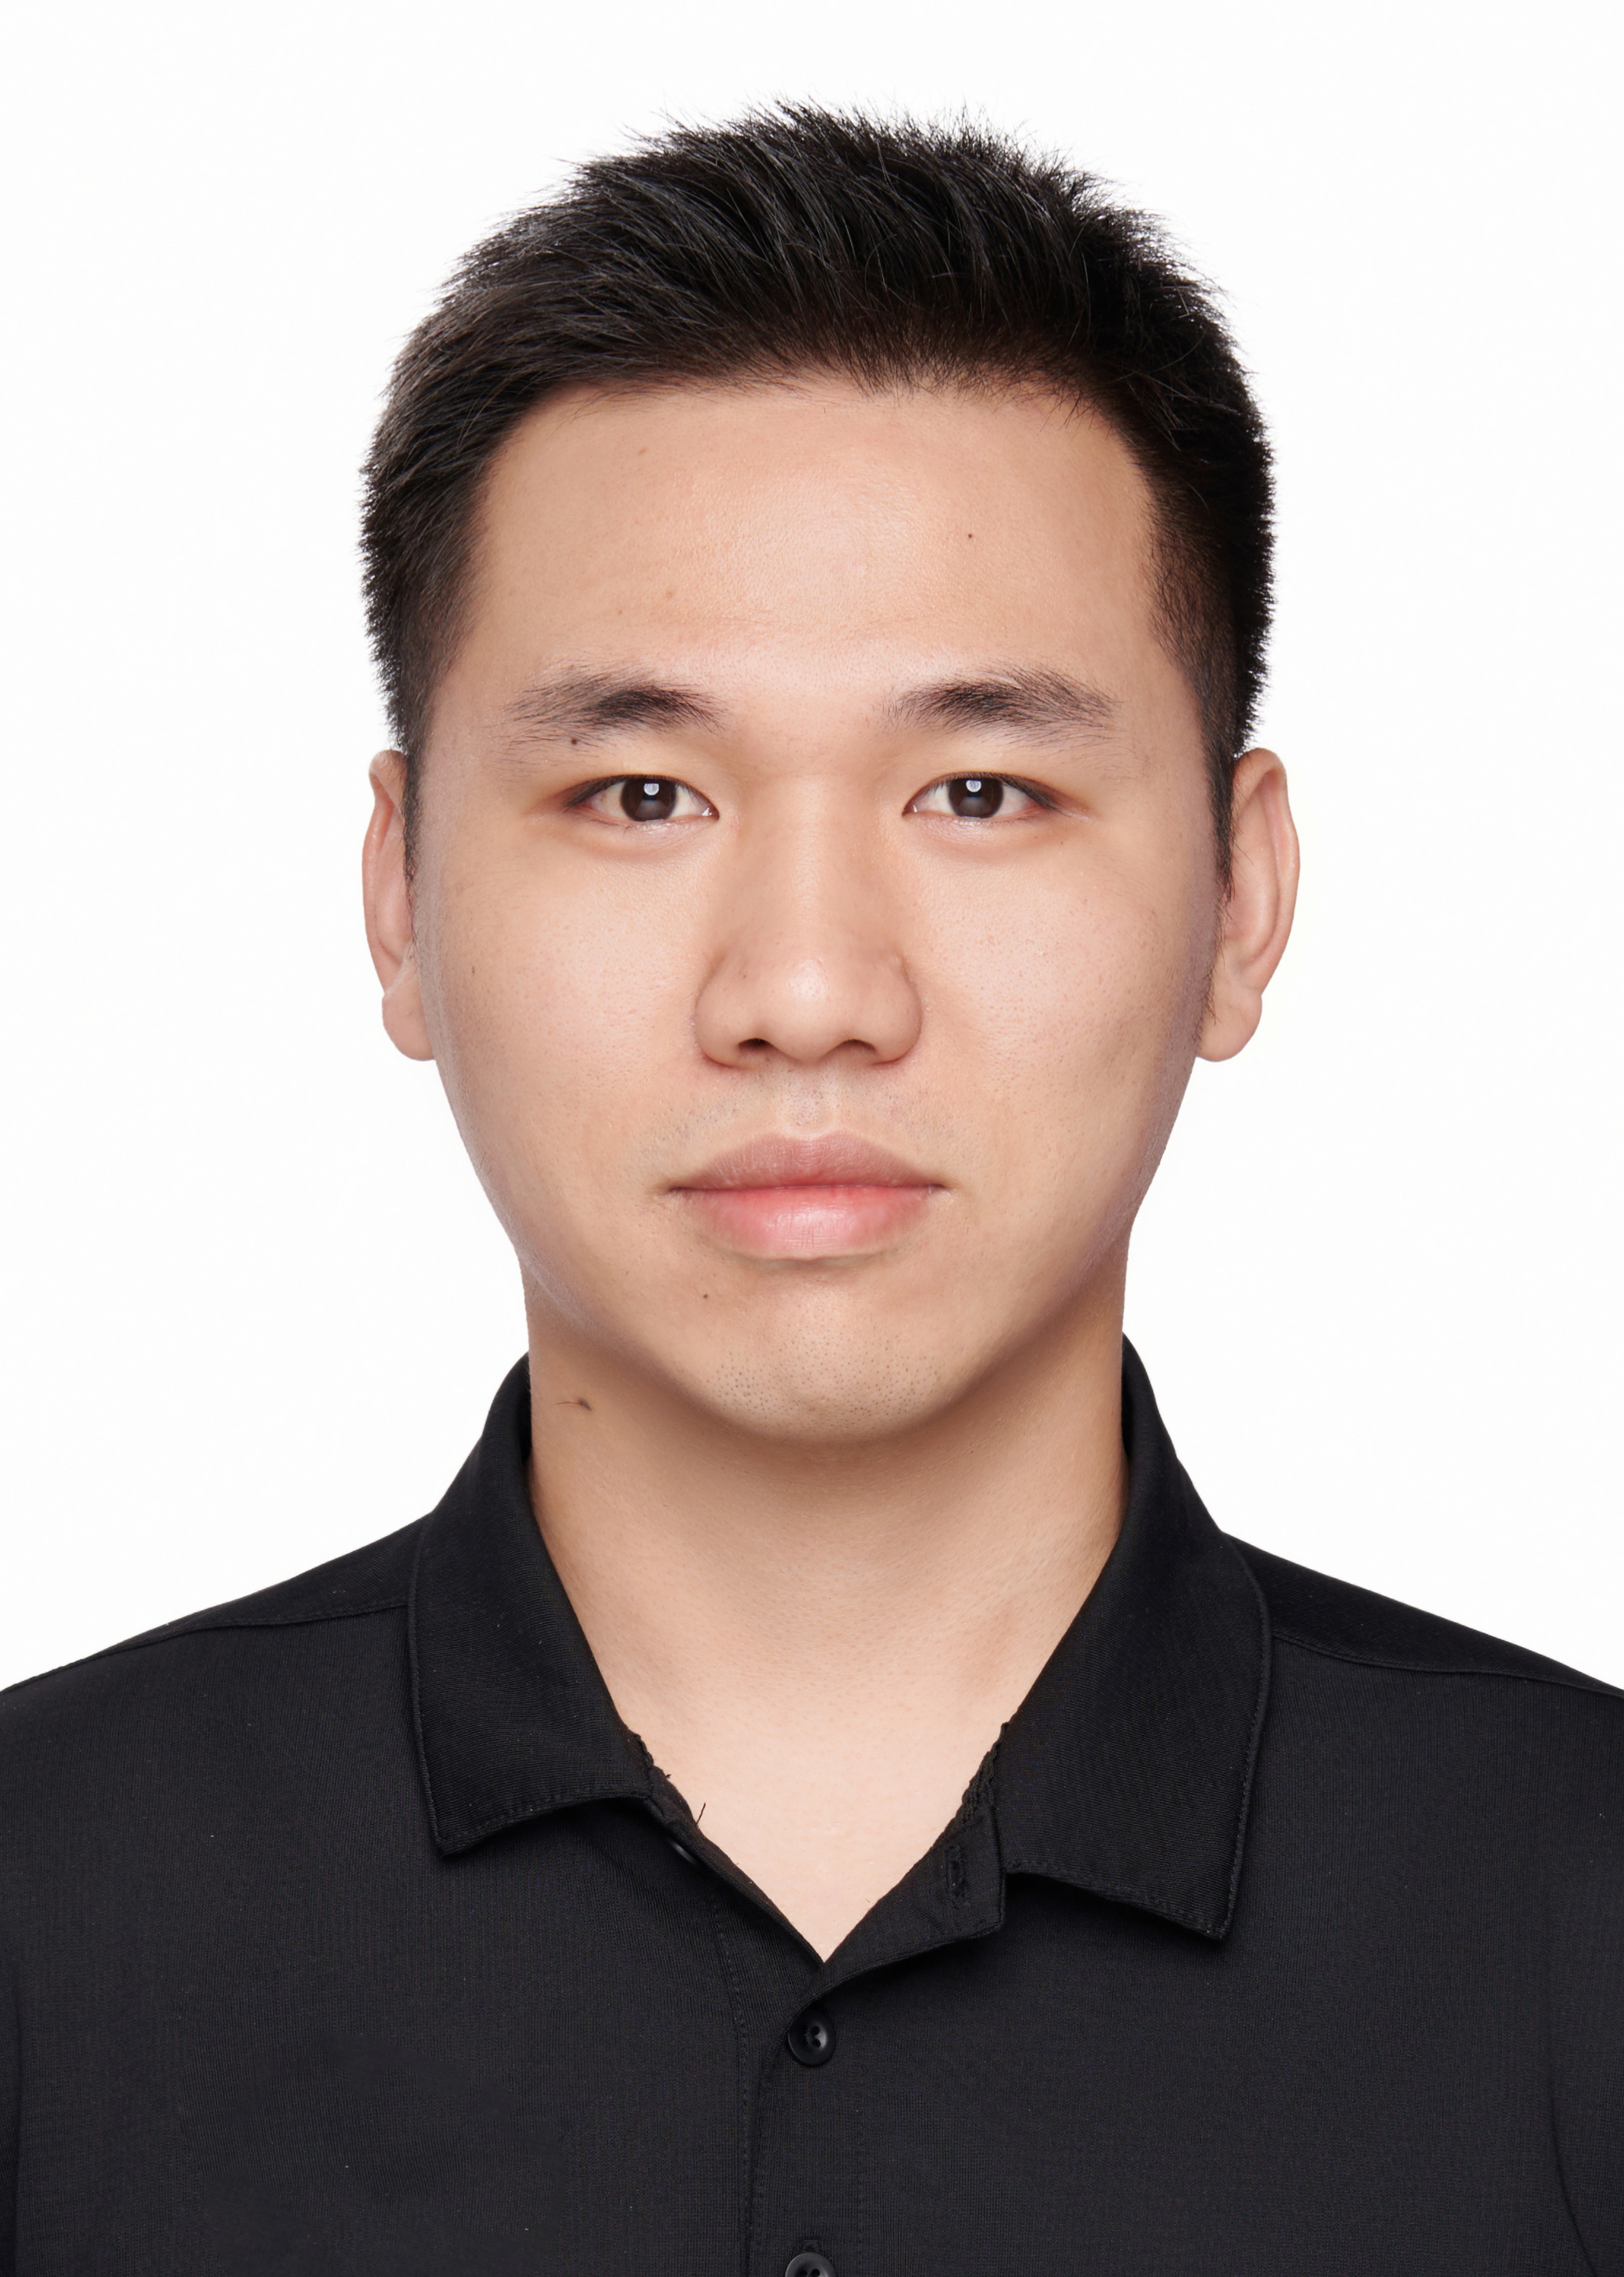
\includegraphics[width=0.92\linewidth]{fig.jpg}
\end{minipage}

\section{个人优势}
小红书技术博主（粉丝 1000+）；零豹 AI 工作室创始人，带领团队从 0 到 1 打造具身智能技术方案。

\section{教育背景}
\datedsubsection{\textbf{合肥工业大学}，卓越工程师学院，电子信息 \textit{博士}}{2025.09 -- 2029.06}
\datedsubsection{\textbf{湖南科技大学}，计算机科学与工程学院，计算机科学与技术，\textit{硕士}}{2022.09 -- 2025.06}
\datedsubsection{\textbf{湖北工业大学}，计算机学院，软件工程，\textit{本科}}{2018.09 -- 2022.06}

\section{科研成果}
\begin{itemize}
  \item \textit{HCA-VLA: Hierarchical Cross-Modal Alignment with Chain-of-Thought Physical Reasoning for Vision–Language–Action Models}. IEEE Transactions on Robotics (TRO，CCF A 顶刊在审) (本人一作)
  \item \textit{VLM-KG: Semantic-Guided 6-DoF Robotic Grasping for Industrial Components via Vision-Language Models and Keypoint-Based Learning}. Robotics and Computer-Integrated Manufacturing (一区Top在审) (本人一作)
  \item \textit{KS-GNN: Keyword Search via Graph Neural Network for Web API Recommendation}. IEEE Transactions on Network and Service Management (IEEE TNSM) (二区，导师一作，本人二作), 2024.
  \item 另外有CCF C会议两篇，Trans期刊一篇，均为本人一作.
\end{itemize}

\section{科研项目}
\datedsubsection{\textbf{空间智能体系与基础研究中心开放基金课题} | 重点课题（10w） | 项目骨干}{2025.02 -- 2025.11}
\begin{itemize}
  \item 负责 VLA 模型训练、微调与多平台部署，涵盖 Pi0、Pi0.5、GR00T、ACT 等模型。
  \item 在 Franka、UR、Aubo、G1 等真机完成落地，覆盖数据采集与格式转换、模型微调、控制代码开发。
  \item 实现异步推理与 RTC 推理，完成机器人端实时控制和多平台适配。
\end{itemize}

\datedsubsection{\textbf{高端装备制造全过程的复杂系统建模与业务互联方法} | 国家重点研发计划“战略性科技创新合作 ”重点专项项目（300w） | 项目参与}{2025-01 -- 2027-12}
\begin{itemize}
  \item 开发基于 VR 的机器人与机械臂控制系统，实现手部坐标与机械臂坐标对齐转换。
  \item 基于机器人 URDF 文件进行 IK 解算，并实时发布角度控制机器人运动。
  \item 支持一个 VR 控制多种异构机器人进行数据采集，掌握 ROS、机械臂运动学、Kinect 等关键技术。
\end{itemize}

\section{实习经历}
\datedsubsection{\textbf{方心科技股份有限公司} | HPC 算法}{2024.09 -- 2024.12}
\begin{itemize}
  \item 负责端侧视觉模型的压缩、转换与部署优化，基于 ONNX/TensorRT/TensorRT-LLM 实现高效推理加速。
\end{itemize}

\datedsubsection{\textbf{深圳华大基因科技有限公司} | NLP 算法}{2024.06 -- 2024.09}
\begin{itemize}
  \item 参与医学多组学研究，负责文本特征提取方法调研与迁移，并协助大模型应用与项目方案整理。
\end{itemize}

\section{荣誉/奖项}
{\small
\begin{tabular}{@{}p{0.48\textwidth} p{0.48\textwidth}@{}}
2022 年硕士国家奖学金 & 2023 年硕士国家奖学金 \\
第二十七届中国机器人及人工智能大赛全国总决赛优秀奖、省赛二等奖 & 第一届湖南省研究生计算机创新大赛三等奖 \\
2023 年湖南省研究生科研创新项目结题 \\
\end{tabular}
}

\section{资格证书}
CET-6 \textperiodcentered\ CET-4 \textperiodcentered\ CCF CSP 认证
\end{document}
